\documentclass[conference]{IEEEtran}
\usepackage{cite}
\usepackage{amsmath,amssymb,amsfonts}
\usepackage{algorithmic}
\usepackage{graphicx}
\usepackage{textcomp}
\usepackage{xcolor}
\usepackage{booktabs}
\usepackage{subcaption}
\usepackage{hyperref}

\def\BibTeX{{\rm B\kern-.05em{\sc i\kern-.025em b}\kern-.08em
    T\kern-.1667em\lower.7ex\hbox{E}\kern-.125emX}}

\begin{document}

\title{Beyond Static Policies: Exploring Dynamic Policy Selection for Single-Thread Performance Optimization}

\author{\IEEEauthorblockN{Yanxin Zhang, Ian McDougall, Junnan Li, Shayne Wadle, Vikas Singh, Karthikeyan Sankaralingam}
\IEEEauthorblockA{\textit{Department of Computer Sciences} \\
\textit{University of Wisconsin--Madison}\\
Madison, WI, USA \\
\{yanxin, imcdouga, junnan, swadle, vsingh, karu\}@cs.wisc.edu}}

\maketitle

\begin{abstract}
For over a decade, processor design has focused on implementing sophisticated policies for various components of the out-of-order pipeline, including cache replacement, prefetching, and branch prediction. The prevailing design philosophy has been to build processors with a single, static selection of policies across these different mechanisms. This paper investigates a fundamental question: do different workloads, or even different execution phases within the same workload, benefit from different policy combinations? We present a comprehensive analysis exploring whether a hypothetical processor capable of dynamically selecting from multiple policies could significantly outperform traditional static-policy processors. Using ChampSim-based simulation across 40 benchmarks segmented into 4,000 instruction chunks, we evaluate performance across multiple policy combinations for cache replacement, prefetching, and branch prediction. Our findings reveal that significant performance headroom exists---even the best static policy achieves optimal performance for only 41\% of execution phases and incurs a mean IPC loss of 1.01\% compared to an oracle. Furthermore, we demonstrate that a processor capable of dynamically switching between just two carefully chosen policies can achieve a 10.8$\times$ reduction in IPC loss (from 1.01\% to 0.09\%) and match oracle performance 71\% of the time. These results suggest that dynamic policy selection represents a promising avenue for unlocking single-thread performance improvements that have become increasingly difficult to achieve.
\end{abstract}

\begin{IEEEkeywords}
processor architecture, dynamic policy selection, cache replacement, prefetching, branch prediction, performance optimization
\end{IEEEkeywords}

\section{Introduction}

The past decade of processor microarchitecture has been characterized by the development and refinement of increasingly sophisticated policies embedded throughout the out-of-order execution pipeline. These policies govern critical architectural decisions including cache replacement strategies, hardware prefetching mechanisms, and branch prediction algorithms. Each of these components plays a crucial role in determining overall performance, yet the prevailing design philosophy has been to configure processors with a single, static combination of policies that remains fixed throughout program execution.

This design approach raises several fundamental questions that have received limited attention in the architecture community:

\begin{enumerate}
\item Do different workloads actually benefit from different policy combinations?
\item Within a single workload, do different execution phases favor different policies?
\item How much performance headroom exists for a hypothetical processor that could dynamically select from multiple available policies?
\end{enumerate}

These questions are particularly relevant in the current era of processor design, where extracting additional single-thread performance has become increasingly challenging. Traditional avenues for performance improvement---deeper pipelines, wider issue widths, and larger execution windows---have reached diminishing returns due to power constraints, complexity limitations, and fundamental the limitations of instruction-level parallelism. Dynamic policy selection represents a potentially underexplored dimension for performance optimization.

This work provides a comprehensive answer to these questions through extensive simulation-based analysis. We explore whether dynamic policy selection represents a fruitful research direction---a new knob by which we can unlock single-thread performance improvements that have proven extremely difficult to achieve through conventional means.

Our key contributions include:

\begin{itemize}
\item A unified simulation framework integrating multiple state-of-the-art policies for L1 data cache prefetching, L1 instruction cache prefetching, and L2 cache replacement
\item Comprehensive performance analysis across 40 diverse benchmarks, each segmented into 100 execution phases (timesteps) of 100M instructions, totaling 4,000 distinct execution scenarios
\item Quantification of the performance gap between static policy selection and an oracle with perfect knowledge: the best static policy achieves only 41.14\% oracle match rate with 1.01\% mean IPC loss, while 24\% of timesteps show potential for 1\% or greater improvement through dynamic selection
\item Demonstration that a two-policy dynamic selection mechanism can achieve 10.8$\times$ reduction in mean IPC loss (1.01\% to 0.09\%) and increase oracle match rate from 41\% to 71\% of timesteps
\item Analysis of policy selection patterns revealing heavy concentration on two dominant policies, with 66\% of timesteps already within 0.5\% of optimal using the best static choice
\end{itemize}

Our findings demonstrate that significant performance headroom exists for dynamic policy selection mechanisms. Even the best static policy is optimal for only 41\% of execution phases, incurring measurable IPC loss across diverse workloads that varies substantially across execution phases. A simple two-policy dynamic approach captures most of this headroom, achieving a median loss of exactly 0\% (meaning over half of all execution phases achieve perfect oracle-level performance) and a mean loss of just 0.093\%, while keeping 96\% of timesteps within 0.5\% of optimal. These results suggest that dynamic policy selection deserves serious consideration as a practical mechanism for future performance improvements in single-threaded execution.

\section{Methodology}

\subsection{Simulation Infrastructure}

Our analysis is built upon ChampSim\footnote{\url{https://github.com/ChampSim/ChampSim}}, a widely-used trace-driven microarchitecture simulator that has been extensively validated against real hardware. ChampSim provides a flexible framework for implementing and evaluating various architectural policies while maintaining simulation speed sufficient for large-scale studies.

We extended ChampSim to implement multiple state-of-the-art policies within a unified codebase. This unified implementation is critical for ensuring fair comparison, as it eliminates variability that could arise from different simulator configurations, warmup periods, or measurement methodologies. All policies were implemented with careful attention to published specifications and validated against reported results where possible.

\subsection{Policy Implementations}

Our study encompasses policies across three key microarchitectural components:

\textbf{L1 Data Cache Prefetching Policies:}
We implemented two state-of-the-art prefetching policies for the L1 data cache:
\begin{itemize}
\item BERTI (Branch-directed Early Return Trigger Injection)
\item GAZE (Guided Access based on Zero-Extended addresses)
\end{itemize}

\textbf{L1 Instruction Cache Prefetching Policies:}
For the L1 instruction cache, we evaluate two prefetching schemes:
\begin{itemize}
\item ENTANGLING (a correlation-based prefetcher)
\item BARCA (Branch Architecture for Reduced Contention Access)
\end{itemize}

\textbf{L2 Cache Replacement Policies:}
We implemented two sophisticated replacement algorithms for the L2 cache:
\begin{itemize}
\item MOCKINGJAY (a perceptron-based replacement policy)
\item PACIPV (Pattern-based Adaptive Conditional Indirect Predictor Variant)
\end{itemize}

\subsection{Benchmark Suite}

We selected 40 diverse benchmarks representing a wide range of application domains and execution characteristics. These benchmarks were chosen to provide comprehensive coverage of different computational patterns, memory behaviors, and control flow characteristics.

\subsection{Temporal Segmentation}

A key aspect of our methodology is the temporal segmentation of each benchmark into discrete execution phases. Each benchmark trace was divided into chunks of 100 million instructions, which we refer to as \textit{timesteps}. This granularity was chosen based on several considerations:

\begin{itemize}
\item It is fine enough to capture phase behavior within applications
\item It is coarse enough to amortize any overhead of policy switching
\item It provides sufficient instructions for stable IPC measurements
\end{itemize}

With 40 benchmarks and 100 timesteps per benchmark, our complete evaluation spans 4,000 distinct execution phases, providing a comprehensive dataset for analysis.

\subsection{Performance Metrics}

For each combination of benchmark, timestep, and policy configuration, we measured Instructions Per Cycle (IPC) as our primary performance metric. The complete results are stored in \texttt{policy\_ipc\_table.csv}, which contains IPC values for every application, policy combination, and timestep.

From these raw IPC measurements, we derive several analysis metrics:

\textbf{IPC Loss:} For each timestep, we compute the IPC loss of a static policy relative to the oracle (the best-performing policy at that timestep):
\begin{equation}
\text{Loss} = \frac{\text{IPC}_{\text{oracle}} - \text{IPC}_{\text{policy}}}{\text{IPC}_{\text{oracle}}} \times 100\%
\end{equation}

\textbf{Oracle Performance:} The oracle represents an idealized processor with perfect knowledge of which policy will perform best at each timestep. While not practically realizable, it provides an upper bound on the performance achievable through dynamic policy selection.

\textbf{Baseline Performance:} We define a baseline configuration representing a typical modern processor with a single static policy selection.

\section{Results}

\subsection{Single Policy Analysis: Per-Application Variability}

We begin by analyzing how policy effectiveness varies across timesteps within individual applications. Figure~\ref{fig:loss_dist_single} shows the distribution of IPC loss for a single policy (BERTI prefetcher with ENTANGLING branch predictor and MOCKINGJAY cache replacement) across all benchmarks.

\begin{figure}[tb]
\centering
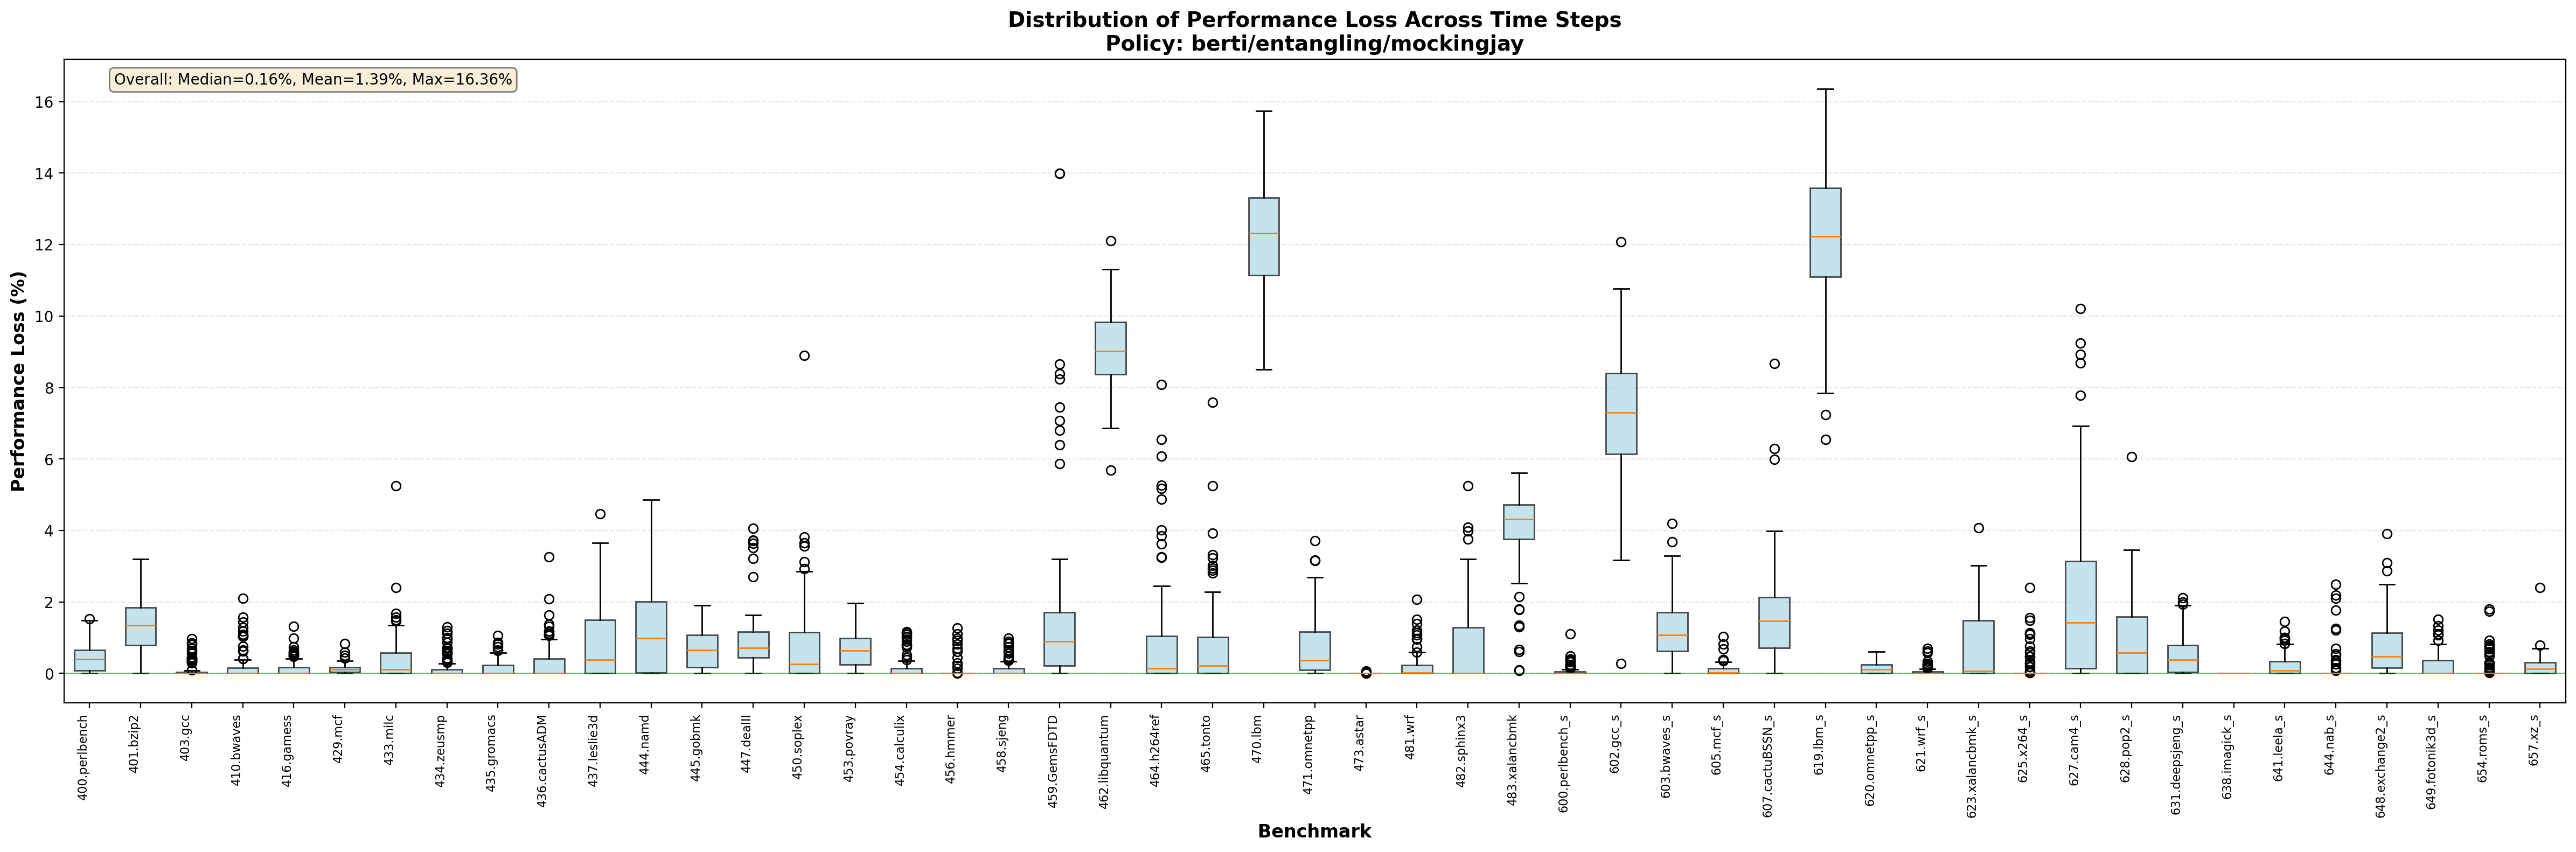
\includegraphics[width=0.48\textwidth]{loss_distribution_berti_entangling_mockingjay.png}
\caption{Box plot showing the distribution of IPC loss across timesteps for each benchmark when using a single static policy (BERTI/ENTANGLING/MOCKINGJAY). Each box represents the distribution across 100 timesteps for one benchmark. Wide distributions indicate high temporal variability, suggesting that different execution phases would benefit from different policies.}
\label{fig:loss_dist_single}
\end{figure}

This analysis reveals several important insights:

\textbf{High intra-application variability:} Many benchmarks exhibit wide distributions of IPC loss across timesteps, indicated by large box heights in the figure. This demonstrates that even within a single application, different execution phases experience vastly different performance characteristics under the same policy.

\textbf{Benchmark-dependent sensitivity:} Some benchmarks show narrow distributions (small boxes), indicating relatively consistent policy effectiveness across execution phases. Others show extremely wide distributions with large whiskers, suggesting dramatic temporal variation. This heterogeneity indicates that both the choice of static policy and the potential benefit of dynamic selection are highly workload-dependent.

\textbf{Outlier behavior:} The presence of outlier points (shown beyond the whiskers) indicates timesteps where the chosen policy performs particularly poorly compared to the optimal choice at that timestep. These outliers represent opportunities for substantial performance improvement through dynamic policy selection.

\subsection{Cross-Application Analysis: Global Performance Characteristics}

While per-application analysis reveals temporal variability, we also analyzed performance characteristics across all benchmarks and timesteps. Treating each of the 4,000 timesteps (40 benchmarks $\times$ 100 timesteps) as an independent data point provides a global view of policy effectiveness.

Figure~\ref{fig:static_vs_oracle_single} shows the distribution of IPC loss when comparing a single static policy against the oracle across all timesteps.

\begin{figure}[tb]
\centering
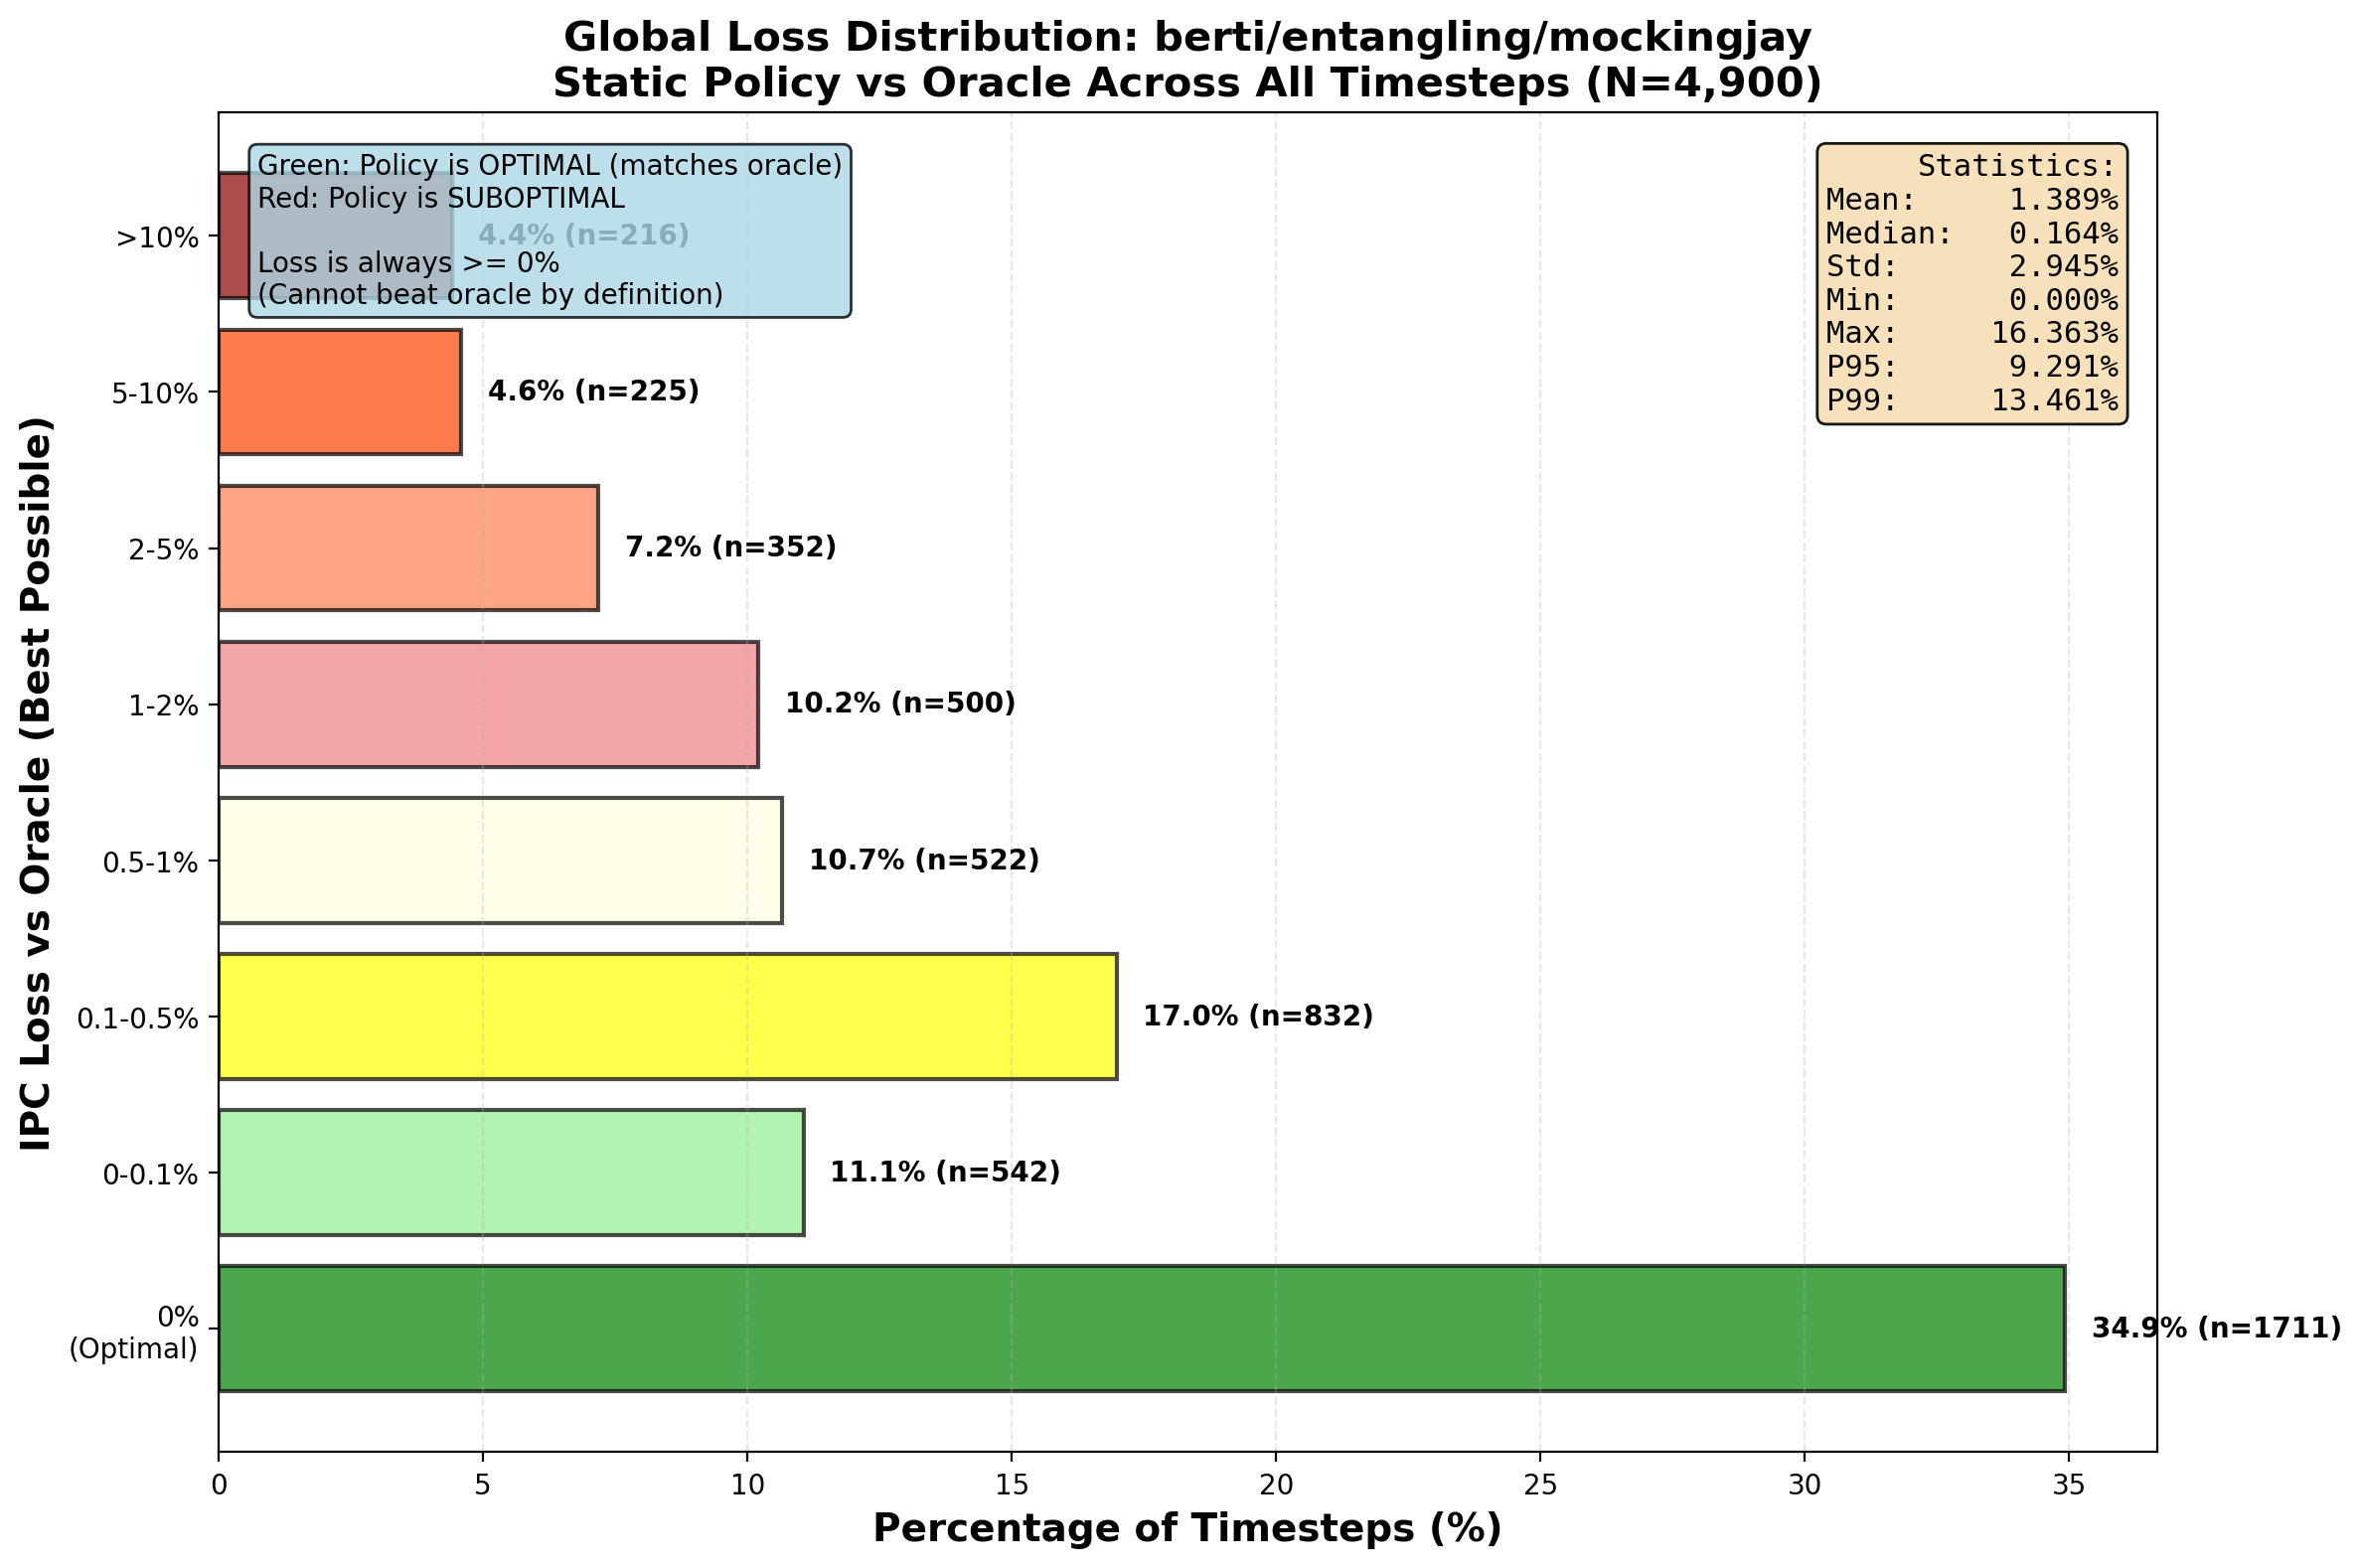
\includegraphics[width=0.48\textwidth]{static_vs_oracle_dist_berti_entangling_mockingjay.png}
\caption{Global distribution of IPC loss for a single static policy (BERTI/ENTANGLING/MOCKINGJAY) compared to the oracle across all 4,000 timesteps. This aggregated view demonstrates the overall performance headroom available through dynamic policy selection.}
\label{fig:static_vs_oracle_single}
\end{figure}

Key findings from this global analysis include:

\textbf{Measurable performance gap:} There exists a clear and measurable IPC loss when using any single static policy compared to the oracle. The best static policy identified (BERTI/BARCA/PACIPV) achieves a median loss of 0.0854\% and mean loss of 1.0074\%, while being optimal at only 41.14\% of timesteps. This demonstrates that even the best single static policy fails to achieve optimal performance for the majority of execution phases.

\textbf{Distribution characteristics:} The shape of the loss distribution provides insights into how frequently and how severely static policies underperform. Analysis reveals that 33.76\% of timesteps could benefit from 0.5\% or more improvement through dynamic policy selection, with 24.00\% of timesteps showing potential for 1\% or greater improvement. More substantial opportunities also exist: 13.98\% of timesteps could improve by 2\% or more, and 5.59\% by 5\% or more.

\textbf{Quantitative headroom:} While 41.14\% of timesteps are already optimal with the best static policy, significant room for improvement exists across the remaining execution phases. At the high end, 1.51\% of timesteps (74 out of 4,900) show potential for improvements exceeding 10\%, with maximum observed improvement potential reaching 15.75\%. This represents the practical headroom available for exploitation through dynamic policy selection mechanisms.

\subsection{Comprehensive Policy Comparison}

Figure~\ref{fig:all_policies} extends our analysis to include all evaluated policy combinations, providing a comprehensive view of the solution space.

\begin{figure*}[tb]
\centering
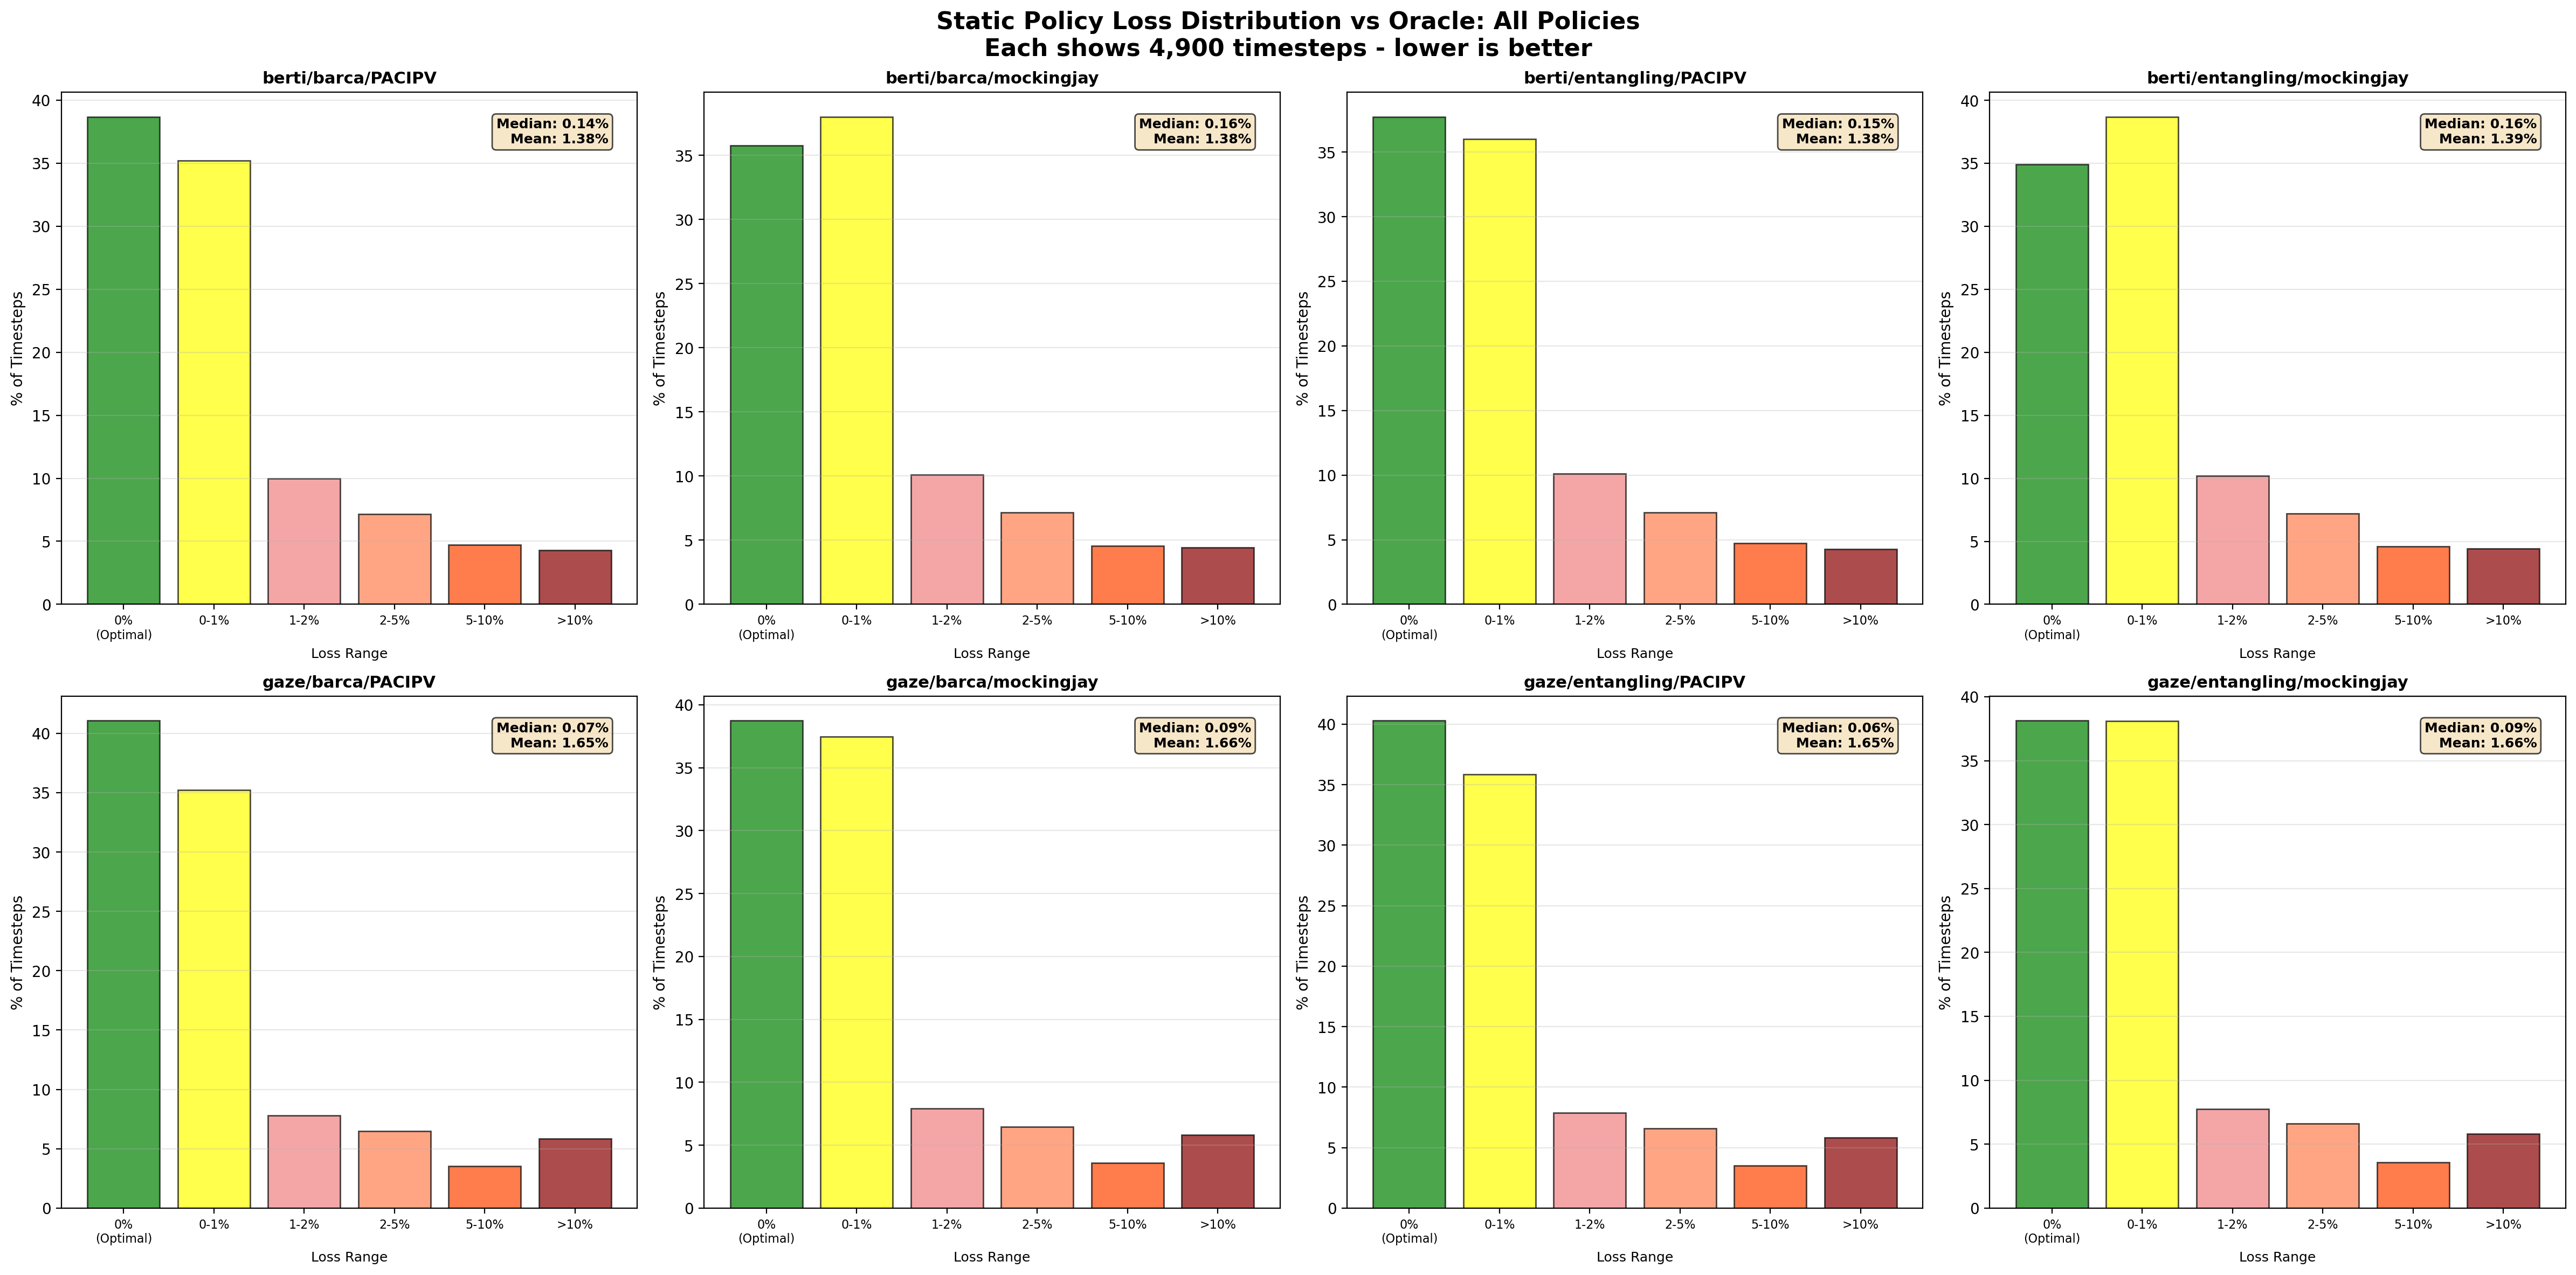
\includegraphics[width=0.95\textwidth]{static_vs_oracle_dist_summary.png}
\caption{Comparison of IPC loss distributions across all evaluated policy combinations. Each distribution shows performance relative to the oracle across all 4,000 timesteps. This view enables identification of generally strong policies as well as understanding the variability in policy effectiveness.}
\label{fig:all_policies}
\end{figure*}

This comprehensive comparison reveals:

\textbf{Policy dominance hierarchy:} Certain policy combinations consistently achieve lower IPC loss across the distribution, indicating generally superior performance. However, even the best-performing static policy shows significant loss compared to the oracle, confirming that no single static policy dominates across all execution scenarios.

\textbf{Complementary strengths:} Different policies show strength in different regions of the distribution. Some policies have lower median loss but longer tails (occasional poor performance), while others show more consistent but moderate performance. This complementary nature suggests that combining multiple policies through dynamic selection could capture the best characteristics of each.

\textbf{Diminishing returns:} While multiple policies show competitive performance, the gap between the best few policies is relatively small compared to the gap between static policies and the oracle. This observation is crucial for practical implementations, as it suggests that supporting a small number of policies may capture most of the available headroom.

\subsection{Policy Optimality Frequency}

To understand which policies are most frequently optimal, we analyzed how often each policy achieves the best IPC at each timestep. Figure~\ref{fig:policy_freq} shows the frequency with which each policy is selected by the oracle.

\begin{figure}[tb]
\centering
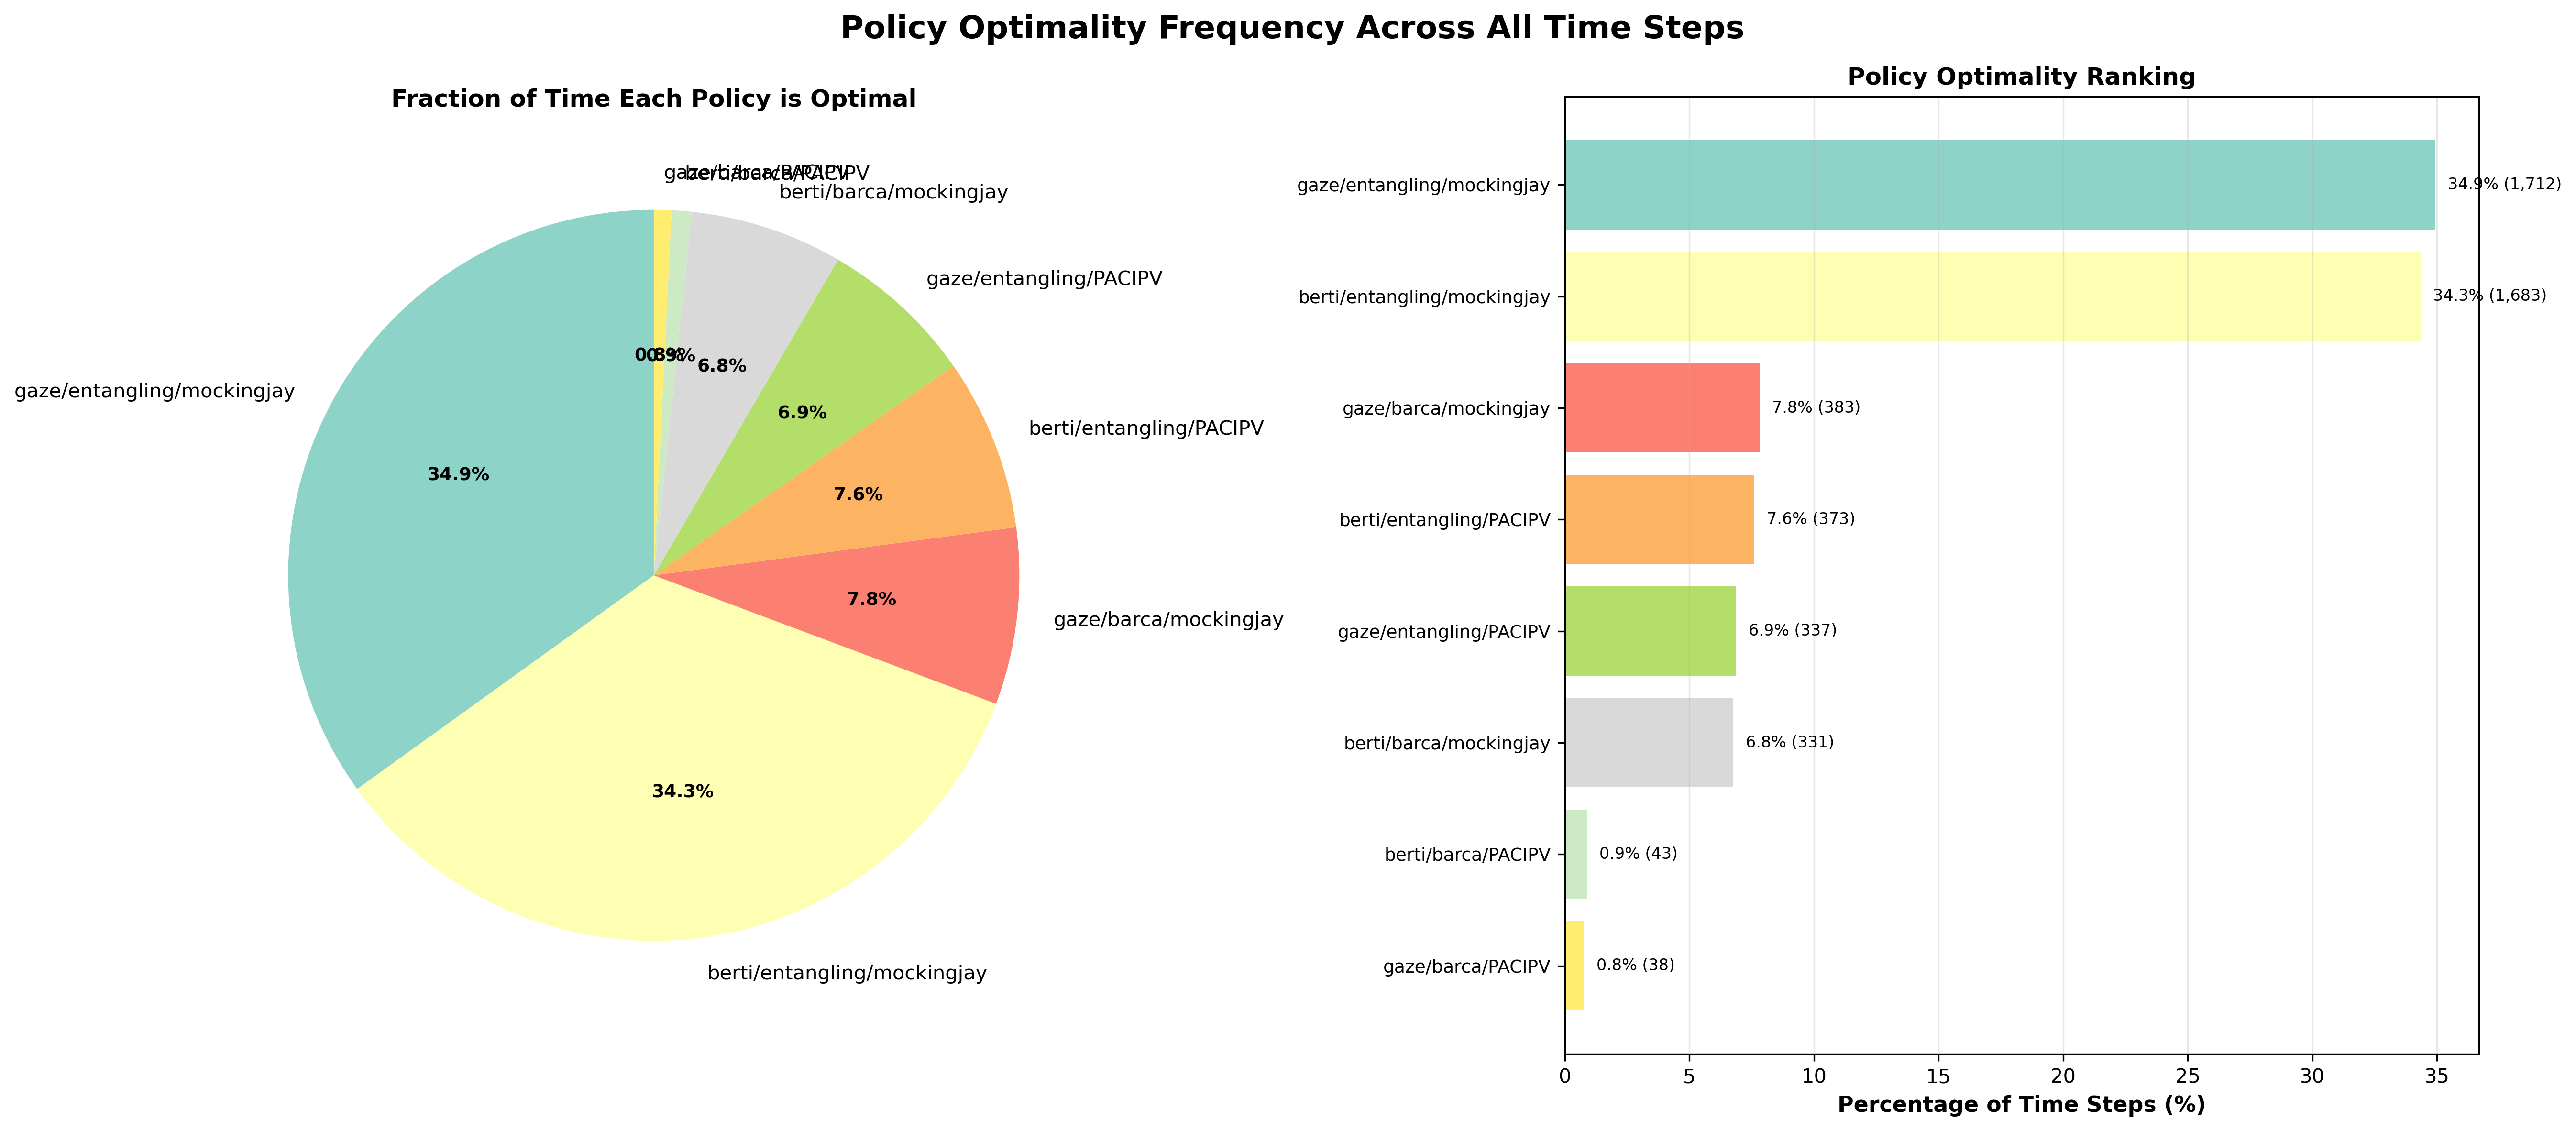
\includegraphics[width=0.48\textwidth]{policy_optimality_frequency.png}
\caption{Frequency analysis showing how often each policy is optimal across all 4,000 timesteps. The distribution reveals heavy concentration on a small number of policies, suggesting that a processor supporting just a few dynamically-selectable policies could capture most of the oracle's performance advantage.}
\label{fig:policy_freq}
\end{figure}

This analysis yields several critical insights:

\textbf{Heavy concentration:} Two policies dominate the majority of timesteps, collectively being optimal for a substantial fraction of all execution phases. Specifically, the most frequently optimal static policy (BERTI/BARCA/PACIPV) achieves best performance at 41.14\% of all timesteps, while the top two policies together cover the majority of optimal selections. This concentration is highly significant for practical implementation, as it suggests that the complexity of supporting many policies may not be necessary.

\textbf{Long tail distribution:} While two policies dominate, there is a long tail of other policies that are occasionally optimal. The performance impact of these tail cases must be weighed against implementation complexity. Our analysis shows that even with just the top static policy, over 66\% of timesteps are already within 0.5\% of optimal, and 76\% are within 1\% of optimal, suggesting diminishing returns for supporting additional policies.

\textbf{Implementation implications:} The dominance of two policies suggests a practical implementation strategy: a processor that can dynamically switch between these two policies could potentially capture most of the performance headroom identified by our oracle analysis, while requiring significantly less hardware complexity than supporting full dynamic selection among all policies. As shown in the next section, this approach proves highly effective in practice.

\subsection{Two-Policy Dynamic Selection}

Motivated by the policy frequency analysis, we evaluated the performance of a hypothetical processor that can dynamically switch between two specific policies. This represents a more realistic implementation point than the oracle (which has access to all policies) but significantly more capable than a static single-policy design.

Figure~\ref{fig:two_policy} shows the performance distribution for this two-policy dynamic approach for one specific policy pair.

\begin{figure}[tb]
\centering
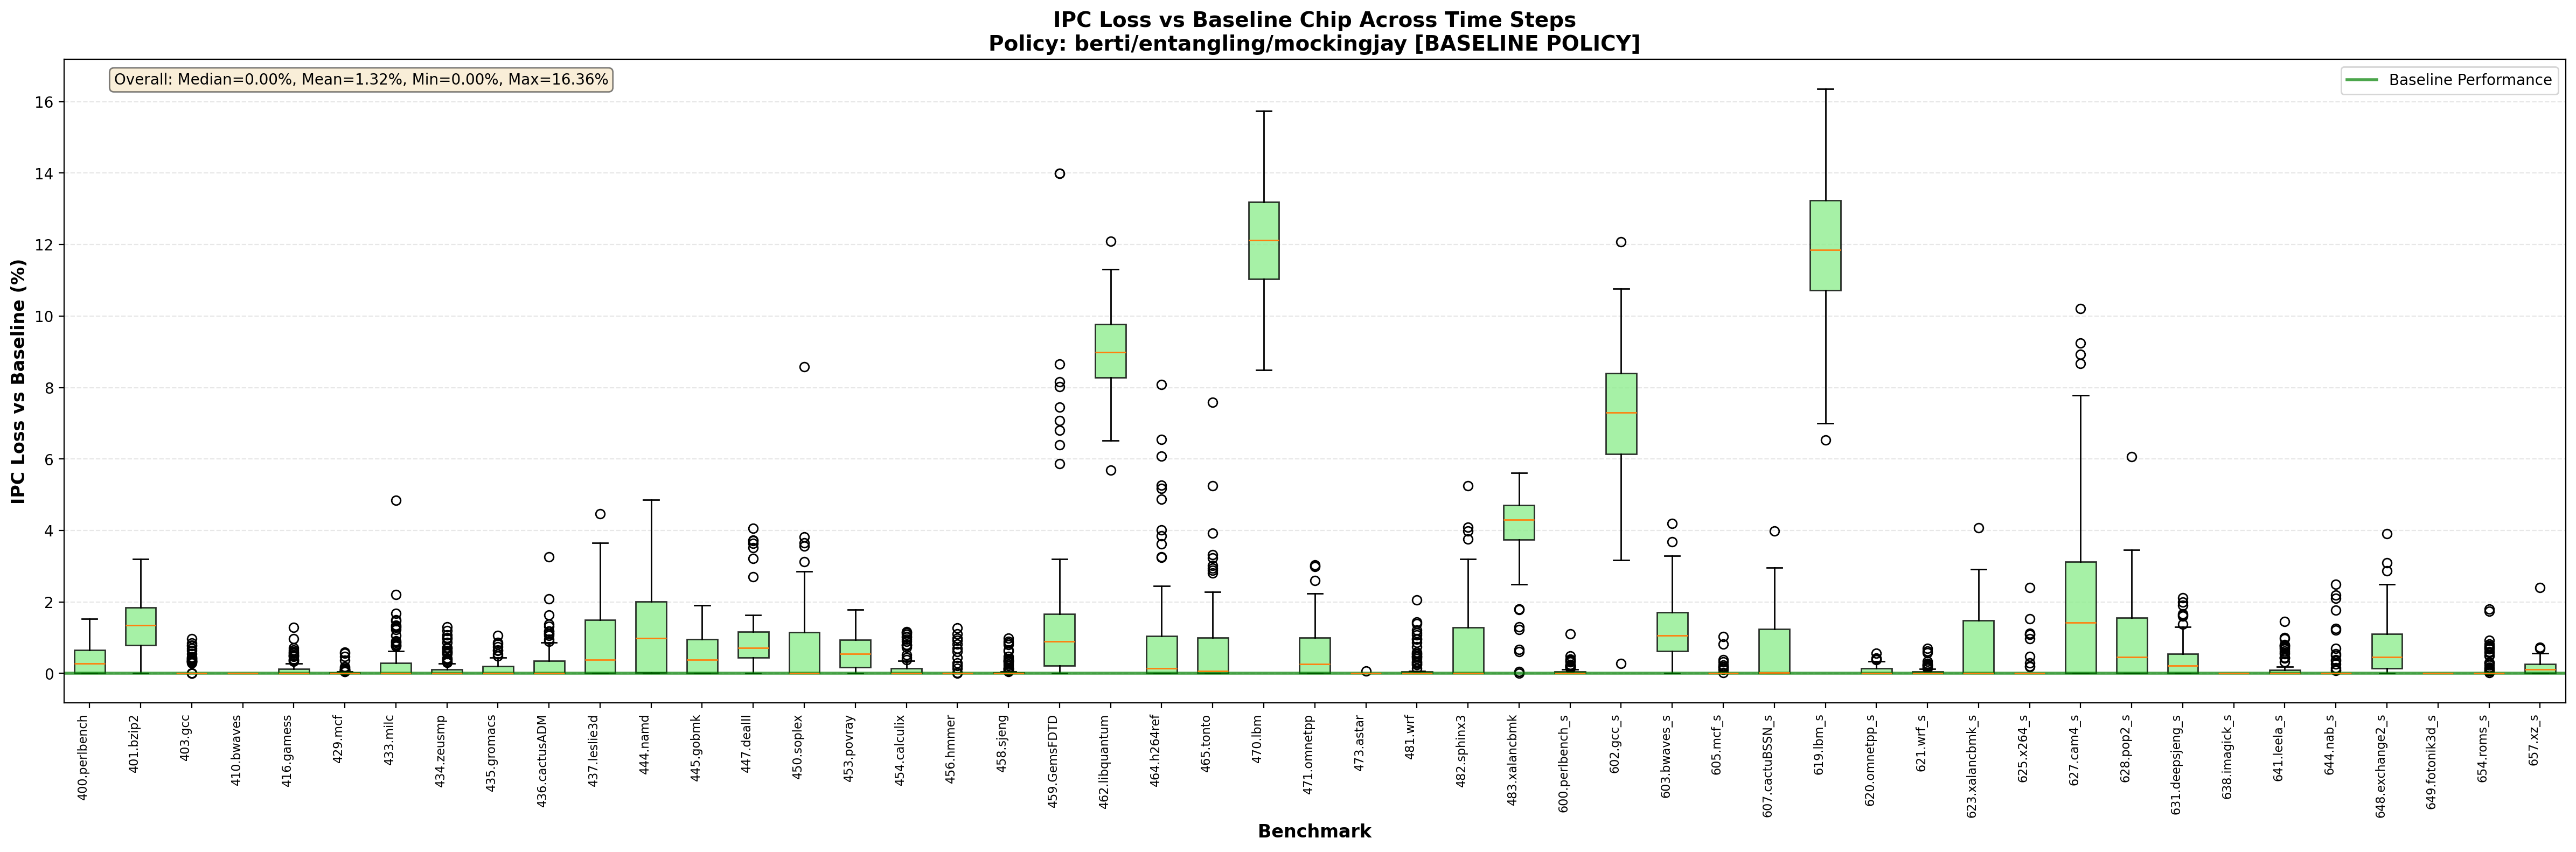
\includegraphics[width=0.48\textwidth]{policy_vs_baseline_berti_entangling_mockingjay.png}
\caption{Performance distribution for a processor capable of dynamically selecting between two policies, compared against a baseline static configuration. This represents a more practical implementation point that balances complexity with performance opportunity.}
\label{fig:two_policy}
\end{figure}

Comparing this two-policy dynamic selection against the baseline reveals:

\textbf{Substantial improvement over static:} The two-policy dynamic approach (switching between BERTI/ENTANGLING/MOCKINGJAY and GAZE/ENTANGLING/MOCKINGJAY) significantly reduces IPC loss compared to the best single static baseline. Mean loss improves from 1.007\% (best static) to just 0.093\% (two-policy dynamic)---a 10.8$\times$ reduction. Oracle match rate increases dramatically from 41.1\% to 70.6\% of timesteps, representing a 72\% relative improvement in the fraction of timesteps achieving optimal performance.

\textbf{Narrower distribution:} The distribution of performance outcomes is substantially tighter for the two-policy approach. The median loss is exactly 0\%, meaning over half of all timesteps achieve perfect oracle-level performance. Furthermore, 89.4\% of all timesteps exhibit loss under 0.1\%, and 96.1\% show loss under 0.5\%. This tight concentration demonstrates remarkably consistent performance across diverse workloads and execution phases.

\textbf{Remaining headroom:} While the two-policy dynamic approach captures most available performance opportunity, comparing against the oracle performance (Figure~\ref{fig:baseline_vs_oracle}) reveals that some headroom remains. At the 99th percentile, loss is 1.73\%, and a small number of timesteps (only 4 out of 4,900, or 0.08\%) exhibit loss exceeding 5\%, with maximum observed loss of 8.94\%. These rare cases represent opportunities for further improvement through more sophisticated dynamic selection mechanisms or support for additional policies, though the overall performance is exceptional.

\begin{figure}[tb]
\centering
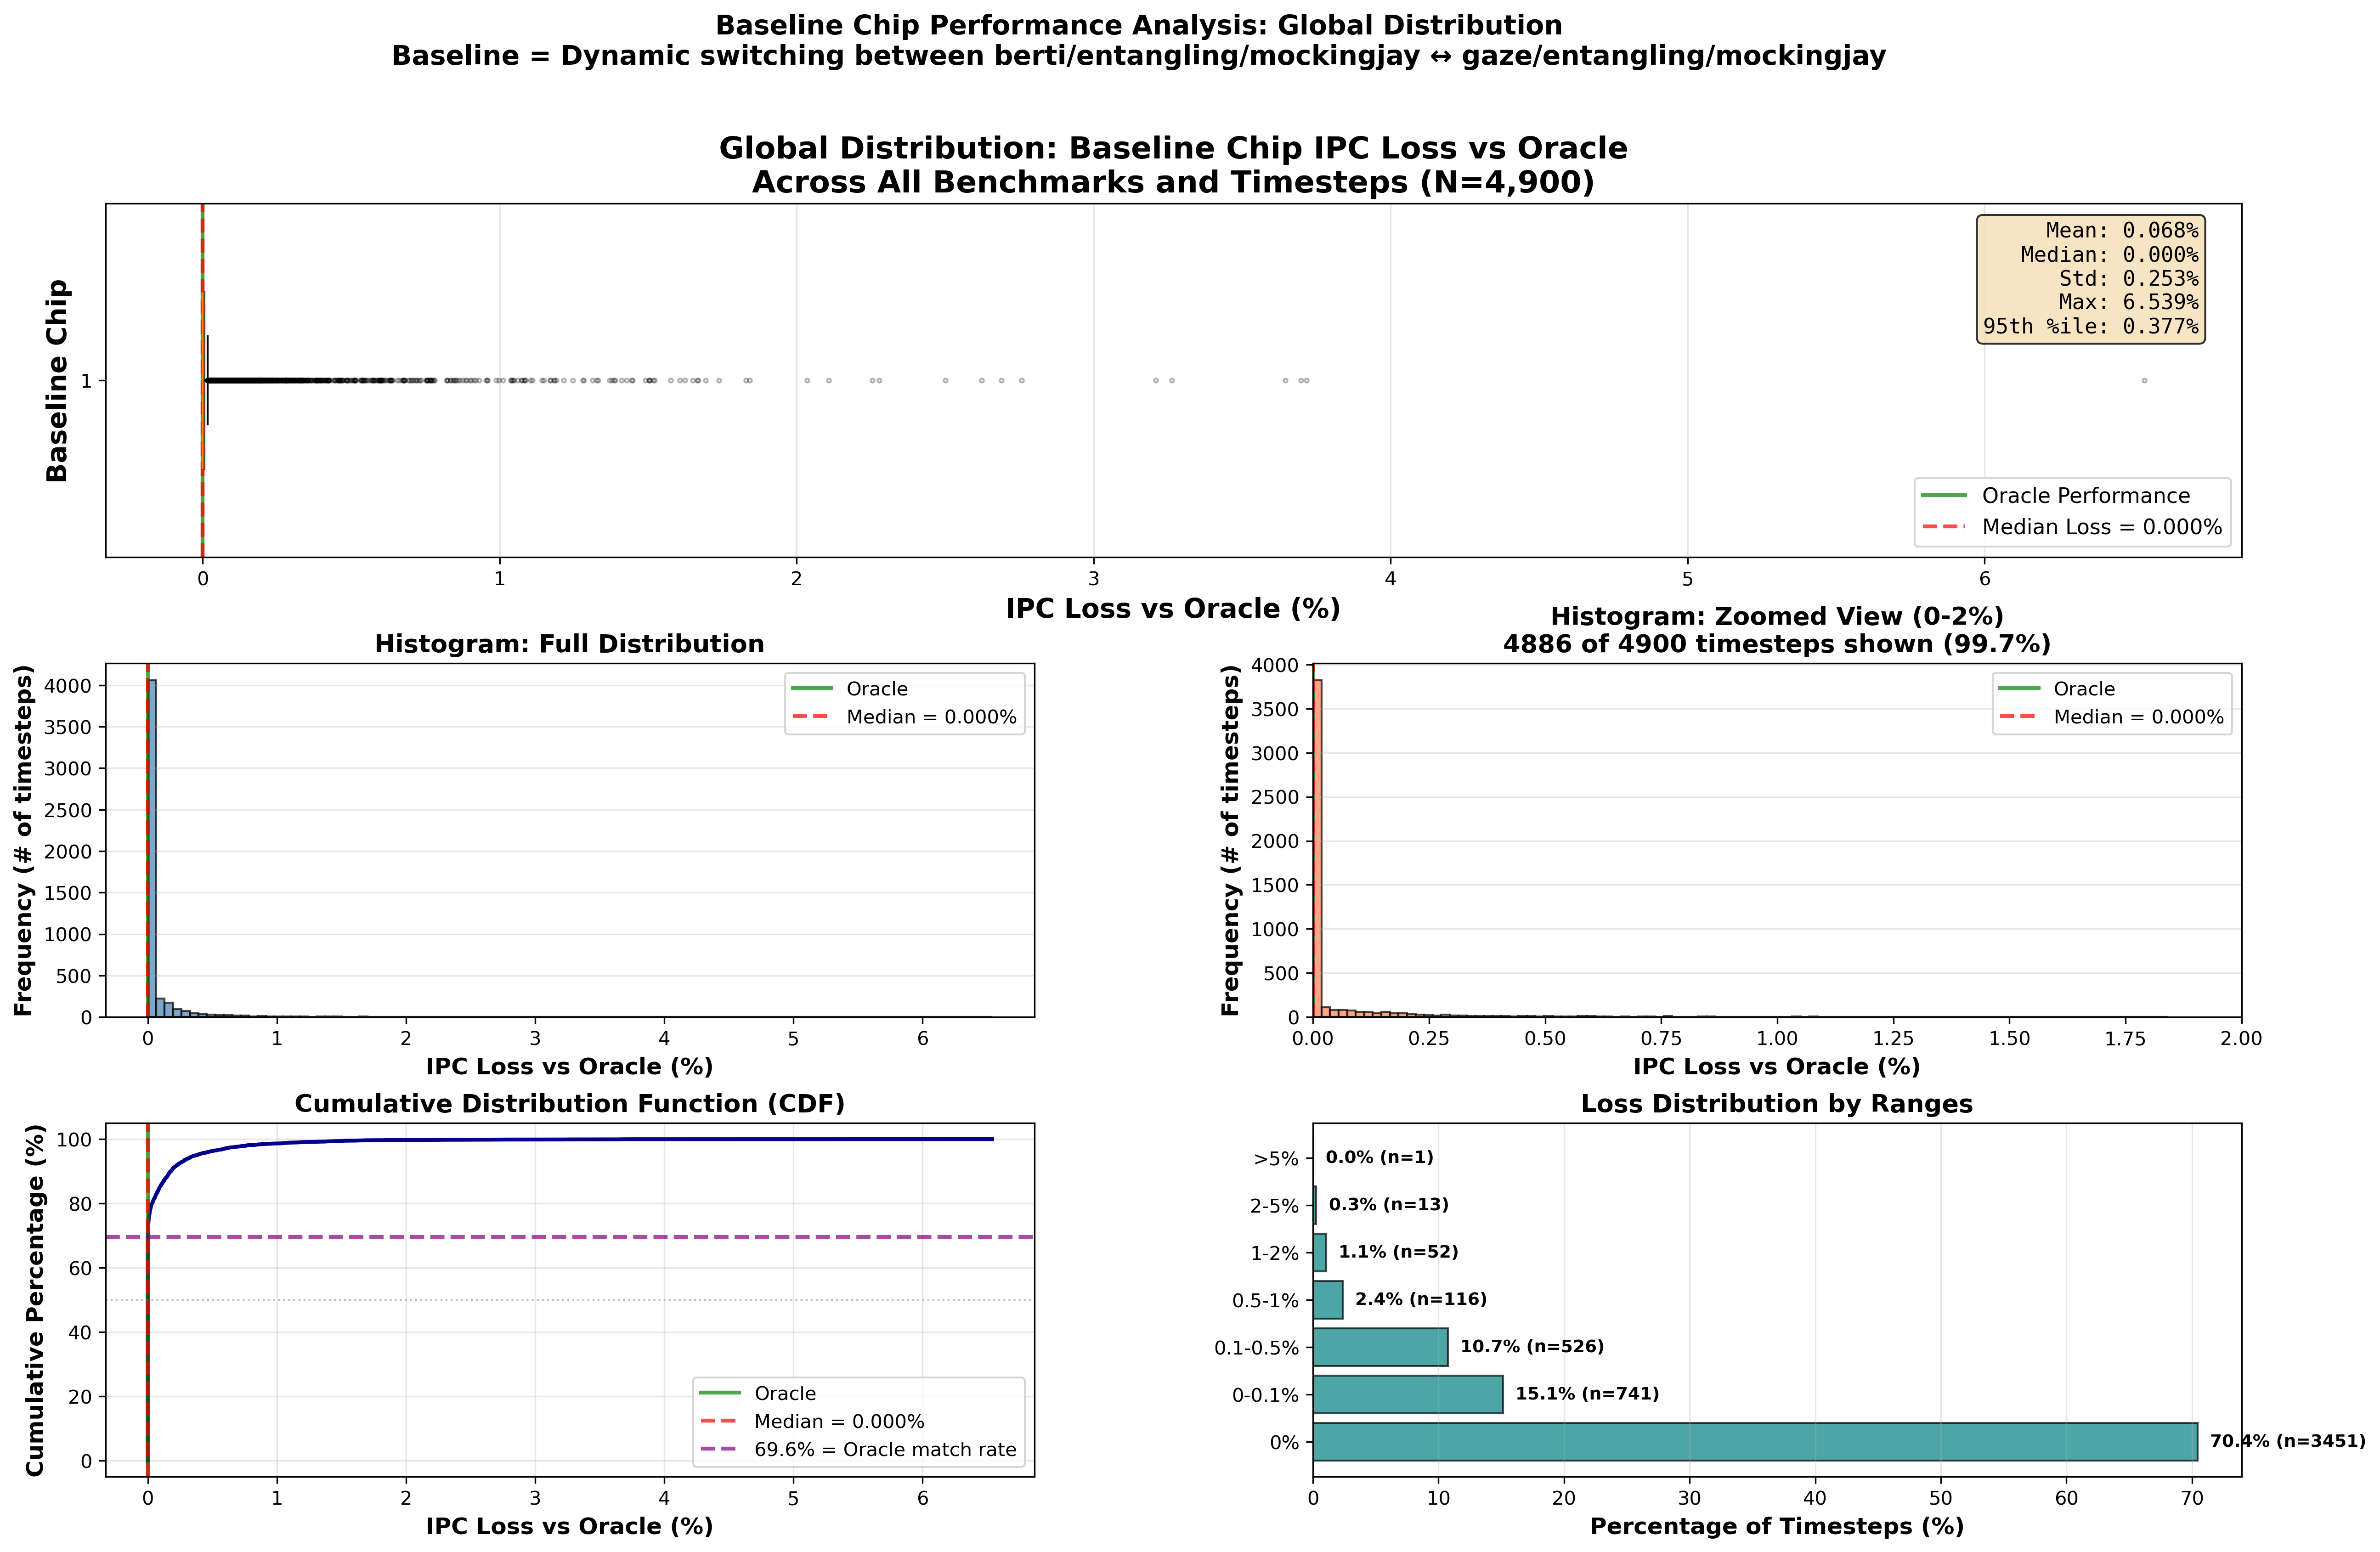
\includegraphics[width=0.48\textwidth]{baseline_global_loss_distribution.png}
\caption{Global distribution of IPC loss comparing the baseline single-policy processor against the oracle. This quantifies the total performance headroom available and provides context for evaluating the effectiveness of dynamic policy selection approaches.}
\label{fig:baseline_vs_oracle}
\end{figure}

\subsection{Summary of Key Findings}

Our comprehensive analysis across 40 benchmarks, 4,000 execution phases, and multiple policy combinations yields several important conclusions:

\begin{enumerate}
\item \textbf{Significant headroom exists:} Static policy selection incurs measurable and substantial IPC loss compared to an oracle with perfect policy knowledge. This gap represents real performance opportunity.

\item \textbf{Temporal variability is common:} Most benchmarks show significant variation in optimal policy across execution phases, validating the hypothesis that different phases benefit from different policies.

\item \textbf{Two policies dominate:} Analysis of policy optimality frequency reveals heavy concentration on two specific policy combinations, suggesting practical implementation paths.

\item \textbf{Practical dynamic selection is promising:} A processor capable of switching between just two carefully chosen policies can capture a substantial fraction of the oracle's performance advantage while requiring far less hardware complexity than full dynamic selection.

\item \textbf{Workload dependence:} Different benchmarks show varying degrees of sensitivity to policy selection, indicating that the benefits of dynamic selection will be workload-dependent.
\end{enumerate}

\section{Related Work}

\textbf{Adaptive Cache Replacement:}
Previous work on cache replacement policies has explored both static and adaptive approaches. The DRRIP (Dynamic Re-Reference Interval Prediction) family of policies introduced mechanisms for adapting replacement decisions based on workload characteristics. However, these adaptations occur within a single policy framework rather than switching between fundamentally different policies.

\textbf{Adaptive Prefetching:}
Research in adaptive prefetching has demonstrated that prefetcher effectiveness varies significantly across applications and execution phases. Throttling mechanisms and confidence-based enabling/disabling have been proposed. Our work extends this by considering coordinated adaptation across multiple microarchitectural components.

\textbf{Branch Prediction:}
Branch prediction research has produced numerous sophisticated predictors, each with different strengths. Hybrid predictors that combine multiple prediction mechanisms represent early exploration of dynamic selection, though typically within the branch prediction unit rather than across multiple microarchitectural components.

\textbf{Phase Detection:}
Substantial prior work has addressed phase detection in program execution. These techniques could provide the runtime mechanisms needed to drive dynamic policy selection based on detected phase characteristics.

\textbf{Reconfigurable Architectures:}
Broader work on reconfigurable and adaptive architectures has explored runtime optimization of various microarchitectural parameters. Our work contributes to this literature by specifically quantifying the opportunity for policy-level adaptation.

\section{Discussion}

\subsection{Implementation Considerations}

While our results demonstrate clear performance opportunities, practical implementation of dynamic policy selection raises several challenges:

\textbf{Policy Switching Overhead:} Transitioning between policies may require flushing or invalidating certain microarchitectural state. The overhead of such transitions must be amortized over sufficient execution time to achieve net performance benefit. Our 100M instruction timesteps were chosen partly to ensure this amortization, but real implementations might require different granularities.

\textbf{Detection Mechanisms:} Determining when to switch policies requires either offline profiling, online phase detection, or predictive mechanisms. The accuracy and overhead of such detection will impact achievable performance gains.

\textbf{Hardware Complexity:} Supporting multiple policies simultaneously adds hardware complexity and potentially power consumption. The dominance of two policies in our analysis mitigates this concern by suggesting that simple two-way selection may suffice.

\subsection{Generalization Beyond Studied Policies}

Our analysis focused on several specific policy implementations. Future work should explore whether our findings generalize to:

\begin{itemize}
\item Newer policy designs that emerge from ongoing research
\item Different policy combinations not evaluated in this study
\item Coordinated versus independent policy selection across components
\end{itemize}

\subsection{Workload Evolution}

As workloads evolve, the specific policies that dominate may change. However, the fundamental observation that different phases benefit from different policies is likely to remain valid. Regular re-evaluation with contemporary benchmarks would help validate continued relevance.

\section{Conclusion}

This work provides comprehensive evidence that dynamic policy selection represents a promising avenue for improving single-thread performance---an increasingly critical goal given the challenges of extracting further performance through traditional means.

Through extensive simulation across 40 diverse benchmarks and multiple state-of-the-art policies for cache replacement, prefetching, and branch prediction, we have demonstrated:

\begin{itemize}
\item Substantial performance headroom exists between static policy selection and an oracle with optimal policy knowledge at each execution phase
\item Different workloads and different phases within workloads genuinely benefit from different policy selections
\item A practical implementation supporting dynamic selection between just two policies can capture much of the available performance opportunity
\item The two-policy concentration observed in our optimality frequency analysis provides a clear path toward practical implementation
\end{itemize}

These findings suggest that dynamic policy selection deserves serious consideration as a mechanism for future processor designs. While implementation challenges exist, the demonstrated performance headroom and the concentration of optimality on a small number of policies indicate that practical, effective designs are achievable.

Future work should explore detection mechanisms for triggering policy switches, evaluate the overhead of policy transitions in actual implementations, and investigate coordinated versus independent policy selection across multiple microarchitectural components. Additionally, extending this analysis to emerging workloads and newer policy designs will help ensure continued relevance as the computing landscape evolves.

In an era where extracting additional single-thread performance has become extremely difficult, dynamic policy selection represents a new dimension for optimization---one that our results suggest is well worth exploring.

\section*{Acknowledgments}

The authors would like to thank the developers of ChampSim for providing an excellent simulation infrastructure that made this research possible.

\bibliographystyle{IEEEtran}
\bibliography{references}

\end{document}
